%%
%% Automatically generated file from DocOnce source
%% (https://github.com/hplgit/doconce/)
%%

% #define PREAMBLE

% #ifdef PREAMBLE
%-------------------- begin preamble ----------------------

\documentclass[%
oneside,                 % oneside: electronic viewing, twoside: printing
final,                   % draft: marks overfull hboxes, figures with paths
10pt,french]{article}

\listfiles               %  print all files needed to compile this document

\usepackage{relsize,makeidx,color,setspace,amsmath,amsfonts,amssymb}
\usepackage[table]{xcolor}
\usepackage{bm,ltablex,microtype}

\usepackage[pdftex]{graphicx}

% Packages for typesetting blocks of computer code
\usepackage{fancyvrb,framed,moreverb}

% Define colors
\definecolor{orange}{cmyk}{0,0.4,0.8,0.2}
\definecolor{tucorange}{rgb}{1.0,0.64,0}
\definecolor{darkorange}{rgb}{.71,0.21,0.01}
\definecolor{darkgreen}{rgb}{.12,.54,.11}
\definecolor{myteal}{rgb}{.26, .44, .56}
\definecolor{gray}{gray}{0.45}
\definecolor{mediumgray}{gray}{.8}
\definecolor{lightgray}{gray}{.95}
\definecolor{brown}{rgb}{0.54,0.27,0.07}
\definecolor{purple}{rgb}{0.5,0.0,0.5}
\definecolor{darkgray}{gray}{0.25}
\definecolor{darkblue}{rgb}{0,0.08,0.45}
\definecolor{darkblue2}{rgb}{0,0,0.8}
\definecolor{lightred}{rgb}{1.0,0.39,0.28}
\definecolor{lightgreen}{rgb}{0.48,0.99,0.0}
\definecolor{lightblue}{rgb}{0.53,0.81,0.92}
\definecolor{lightblue2}{rgb}{0.3,0.3,1.0}
\definecolor{lightpurple}{rgb}{0.87,0.63,0.87}
\definecolor{lightcyan}{rgb}{0.5,1.0,0.83}

\colorlet{comment_green}{green!50!black}
\colorlet{string_red}{red!60!black}
\colorlet{keyword_pink}{magenta!70!black}
\colorlet{indendifier_green}{green!70!white}

% Backgrounds for code
\definecolor{cbg_gray}{rgb}{.95, .95, .95}
\definecolor{bar_gray}{rgb}{.92, .92, .92}

\definecolor{cbg_yellowgray}{rgb}{.95, .95, .85}
\definecolor{bar_yellowgray}{rgb}{.95, .95, .65}

\colorlet{cbg_yellow2}{yellow!10}
\colorlet{bar_yellow2}{yellow!20}

\definecolor{cbg_yellow1}{rgb}{.98, .98, 0.8}
\definecolor{bar_yellow1}{rgb}{.98, .98, 0.4}

\definecolor{cbg_red1}{rgb}{1, 0.85, 0.85}
\definecolor{bar_red1}{rgb}{1, 0.75, 0.85}

\definecolor{cbg_blue1}{rgb}{0.87843, 0.95686, 1.0}
\definecolor{bar_blue1}{rgb}{0.7,     0.95686, 1}

%\setlength{\fboxsep}{-1.5mm}  % adjust cod_vpad/pro_vpad background box

%% Background for code blocks (parameter is color name)

%% pro/cod_vpad: gives some vertical padding before and after the text
%% (but has more simplistic code than _cod/pro_tight+cod/pro).
%% pro/cod_vpad can be used to enclose Verbatim or lst begin/end for code.
%% pro/cod calls _pro/cod_tight and has very little vertical padding,
%% used to enclose Verbatim and other begin/end for code.
%% (pro/cod is what the ptex2tex program could produce with the
%% Blue/BlueBar definitions in .ptex2tex.cfg.)

\newenvironment{cod_vpad}[1]{
   \def\FrameCommand{\colorbox{#1}}
   \MakeFramed{\FrameRestore}}
   {\endMakeFramed}

\newenvironment{_cod_tight}[1]{
   \def\FrameCommand{\colorbox{#1}}
   \FrameRule0.6pt\MakeFramed {\FrameRestore}\vskip3mm}
   {\vskip0mm\endMakeFramed}

\newenvironment{cod}[1]{
\bgroup\rmfamily
\fboxsep=0mm\relax
\begin{_cod_tight}{#1}
\list{}{\parsep=-2mm\parskip=0mm\topsep=0pt\leftmargin=2mm
\rightmargin=2\leftmargin\leftmargin=4pt\relax}
\item\relax}
{\endlist\end{_cod_tight}\egroup}

%% Background for complete program blocks (parameter 1 is color name
%% for background, parameter 2 is color for left bar)
\newenvironment{pro_vpad}[2]{
   \def\FrameCommand{\color{#2}\vrule width 1mm\normalcolor\colorbox{#1}}
   \MakeFramed{\FrameRestore}}
   {\endMakeFramed}

\newenvironment{_pro_tight}[2]{
   \def\FrameCommand{\color{#2}\vrule width 1mm\normalcolor\colorbox{#1}}
   \FrameRule0.6pt\MakeFramed {\advance\hsize-2mm\FrameRestore}\vskip3mm}
   {\vskip0mm\endMakeFramed}

\newenvironment{pro}[2]{
\bgroup\rmfamily
\fboxsep=0mm\relax
\begin{_pro_tight}{#1}{#2}
\list{}{\parsep=-2mm\parskip=0mm\topsep=0pt\leftmargin=2mm
\rightmargin=2\leftmargin\leftmargin=4pt\relax}
\item\relax}
{\endlist\end{_pro_tight}\egroup}

\usepackage{minted}
\usemintedstyle{default}

\usepackage[T1]{fontenc}
%\usepackage[latin1]{inputenc}
\usepackage{ucs}
\usepackage[utf8x]{inputenc}

\usepackage{lmodern}         % Latin Modern fonts derived from Computer Modern

% Hyperlinks in PDF:
\definecolor{linkcolor}{rgb}{0,0,0.4}
\usepackage{hyperref}
\hypersetup{
    breaklinks=true,
    colorlinks=true,
    linkcolor=linkcolor,
    urlcolor=linkcolor,
    citecolor=black,
    filecolor=black,
    %filecolor=blue,
    pdfmenubar=true,
    pdftoolbar=true,
    bookmarksdepth=3   % Uncomment (and tweak) for PDF bookmarks with more levels than the TOC
    }
%\hyperbaseurl{}   % hyperlinks are relative to this root

\setcounter{tocdepth}{2}  % levels in table of contents

% Tricks for having figures close to where they are defined:
% 1. define less restrictive rules for where to put figures
\setcounter{topnumber}{2}
\setcounter{bottomnumber}{2}
\setcounter{totalnumber}{4}
\renewcommand{\topfraction}{0.95}
\renewcommand{\bottomfraction}{0.95}
\renewcommand{\textfraction}{0}
\renewcommand{\floatpagefraction}{0.75}
% floatpagefraction must always be less than topfraction!
% 2. ensure all figures are flushed before next section
\usepackage[section]{placeins}
% 3. enable begin{figure}[H] (often leads to ugly pagebreaks)
%\usepackage{float}\restylefloat{figure}

% --- fancyhdr package for fancy headers ---
\usepackage{fancyhdr}
\fancyhf{} % sets both header and footer to nothing
\renewcommand{\headrulewidth}{0pt}
\fancyfoot[LE,RO]{\thepage}
% Ensure copyright on titlepage (article style) and chapter pages (book style)
\fancypagestyle{plain}{
  \fancyhf{}
  \fancyfoot[C]{{\footnotesize \copyright\ 2019, Ahmed Ammar. Released under CC Attribution 4.0 license}}
%  \renewcommand{\footrulewidth}{0mm}
  \renewcommand{\headrulewidth}{0mm}
}
% Ensure copyright on titlepages with \thispagestyle{empty}
\fancypagestyle{empty}{
  \fancyhf{}
  \fancyfoot[C]{{\footnotesize \copyright\ 2019, Ahmed Ammar. Released under CC Attribution 4.0 license}}
  \renewcommand{\footrulewidth}{0mm}
  \renewcommand{\headrulewidth}{0mm}
}

\pagestyle{fancy}


% prevent orhpans and widows
\clubpenalty = 10000
\widowpenalty = 10000

\newenvironment{doconceexercise}{}{}
\newcounter{doconceexercisecounter}
% --- begin definition of \listofexercises command ---
\makeatletter
\newcommand\listofexercises{\section*{List of Exercises}
\@starttoc{loe}
}
\newcommand*{\l@doconceexercise}{\@dottedtocline{0}{0pt}{6.5em}}
\makeatother
% --- end definition of \listofexercises command ---



% ------ header in subexercises ------
%\newcommand{\subex}[1]{\paragraph{#1}}
%\newcommand{\subex}[1]{\par\vspace{1.7mm}\noindent{\bf #1}\ \ }
\makeatletter
% 1.5ex is the spacing above the header, 0.5em the spacing after subex title
\newcommand\subex{\@startsection{paragraph}{4}{\z@}%
                  {1.5ex\@plus1ex \@minus.2ex}%
                  {-0.5em}%
                  {\normalfont\normalsize\bfseries}}
\makeatother


% --- end of standard preamble for documents ---


\usepackage[french]{babel}

% insert custom LaTeX commands...

\raggedbottom
\makeindex
\usepackage[totoc]{idxlayout}   % for index in the toc
\usepackage[nottoc]{tocbibind}  % for references/bibliography in the toc

%-------------------- end preamble ----------------------

\begin{document}

% matching end for #ifdef PREAMBLE
% #endif

\newcommand{\exercisesection}[1]{\subsection*{#1}}


% ------------------- main content ----------------------



% ----------------- title -------------------------

\thispagestyle{empty}

\begin{center}
{\LARGE\bf
\begin{spacing}{1.25}
TD N°3 : Bibliothèques numpy et matplotlib
\end{spacing}
}
\end{center}

% ----------------- author(s) -------------------------

\begin{center}
{\bf Ahmed Ammar (\texttt{ahmed.ammar@fst.utm.tn})}
\end{center}

    \begin{center}
% List of all institutions:
\centerline{{\small Institut Préparatoire aux Études Scientifiques et Techniques, Université de Carthage.}}
\end{center}
    
% ----------------- end author(s) -------------------------

% --- begin date ---
\begin{center}
Nov 29, 2019
\end{center}
% --- end date ---

\vspace{1cm}


\tableofcontents


\vspace{1cm} % after toc




% !split


% --- begin exercise ---
\begin{doconceexercise}
\refstepcounter{doconceexercisecounter}

\exercisesection{Exercise \thedoconceexercisecounter: Tracer une fonction}


Ecrivez un programme qui trace la fonction $g(y) = e^{-y} sin(4y)$ pour $y \in [0, 4]$ en utilisant une ligne continue rouge. Utilisez 500 intervalles pour évaluer les points dans [0,4]. Stockez toutes les coordonnées et les valeurs dans des tableaux. Placez le texte des graduations sur les axes et utilisez le titre "Onde sinusoïdale atténuée".


% --- begin solution of exercise ---
\paragraph{Solution.}
La programme qui trace la fonction $g(y)$ est:
\begin{pro}{cbg_gray}{bar_gray}\begin{minted}[fontsize=\fontsize{9pt}{9pt},linenos=false,mathescape,baselinestretch=1.0,fontfamily=tt,xleftmargin=2mm]{python}
# Importation
import numpy as np
import matplotlib.pyplot as plt

def g(y):
    return np.exp(-y)*np.sin(4*y)

y = np.linspace(0, 4, 501)
# définir un nouveau graphique
plt.figure()
# tracer la fonction g(y) avec ligne solide rouge
plt.plot(y, g(y), 'r-')
plt.xlabel('y'); plt.ylabel('g(y)')
plt.title(u'Onde sinusoïdale atténuée')
 # sauvgarder le grahique (format PNG et PDF)
plt.savefig("fig_ex1.png"); plt.savefig("fig_ex1.pdf")
# Afficher le graphique
plt.show()
\end{minted}
\end{pro}
\noindent

% --- end solution of exercise ---

\end{doconceexercise}
% --- end exercise ---




% --- begin exercise ---
\begin{doconceexercise}
\refstepcounter{doconceexercisecounter}

\exercisesection{Exercise \thedoconceexercisecounter: Tracer deux fonctions}


Comme Exercice 1, mais ajouter une courbe en pointillé noir pour la fonction $h(y) = e^{-\frac{3}{2}y} sin(4y)$. Inclure une légende pour chaque courbe (avec les noms $g$ et $h$).


% --- begin solution of exercise ---
\paragraph{Solution.}
La programme qui trace la fonction $g(y)$ avec une nouvelle fonction $h(y)$ est:
\begin{pro}{cbg_gray}{bar_gray}\begin{minted}[fontsize=\fontsize{9pt}{9pt},linenos=false,mathescape,baselinestretch=1.0,fontfamily=tt,xleftmargin=2mm]{python}
# Importation
import numpy as np
import matplotlib.pyplot as plt

def g(y):
    return np.exp(-y)*np.sin(4*y)

def h(y):
    return np.exp(-(3./2)*y)*np.sin(4*y)

y = np.linspace(0, 4, 501)
plt.figure()
plt.plot(y, g(y), 'r-', y, h(y), 'k--')
plt.xlabel('y'); plt.ylabel('g(y)')
plt.title(u'Onde sinusoïdale atténuée')
plt.legend(['g', 'h'])

plt.savefig("fig_ex2.png"); plt.savefig("fig_ex2.pdf")
plt.show()
\end{minted}
\end{pro}
\noindent

% --- end solution of exercise ---

\end{doconceexercise}
% --- end exercise ---




% --- begin exercise ---
\begin{doconceexercise}
\refstepcounter{doconceexercisecounter}

\exercisesection{Exercise \thedoconceexercisecounter: Racines d’une équation du second degré}


Dans l'"application de l'exercice 4 dans TD N°2, nous avons montré la représentation graphique d'une équation du second degré $f(x)=0.83x^2+3.8x+2.48$ ainsi que ses racines réelles:



\vspace{6mm}

% inline figure
\centerline{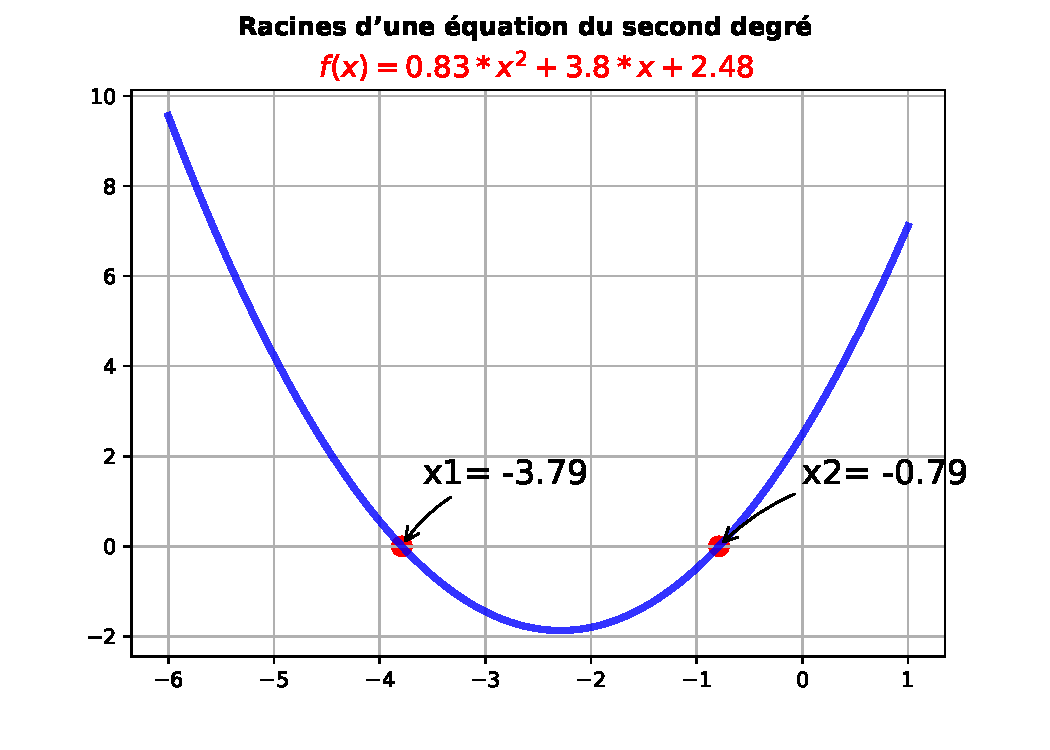
\includegraphics[width=0.7\linewidth]{imgs/equation2deg.pdf}}

\vspace{6mm}


Reproduire ce graphique en utilisant la fonction \texttt{EqSecondDegree(a,b,c)} du script Python \texttt{racines.py} pour déterminer les valeurs des racines x1 et x2 de l’équation $f(x)$.


% --- begin solution of exercise ---
\paragraph{Solution.}
Le programme qui reproduit la figure en utilisant la fonction \texttt{EqSecondDegree()}:

\begin{cod}{cbg_gray}\begin{minted}[fontsize=\fontsize{9pt}{9pt},linenos=false,mathescape,baselinestretch=1.0,fontfamily=tt,xleftmargin=2mm]{python}
# Importation
import numpy as np
import matplotlib.pyplot as plt
from racines import EqSecondDegree
# NOTE: le module racines est le fichier racines.py
# qu'on doit placer dans le répertoire de travail.

def f(x):
    return 0.83 * x**2 + 3.8 * x + 2.48
x = np.linspace(-6, 1, 200)
y = f(x)
x1, x2 = EqSecondDegree(0.83, 3.8, 2.48)

plt.figure(figsize=(7, 5), dpi=80)
plt.plot(x, y, color="blue", linewidth=3, linestyle="-", alpha=.8)
plt.scatter([x1,x2], [f(x1), f(x2)], 80, color='red')

plt.annotate('x1= {:.2f}'.format(x1),
             xy=(x1, f(x1)), xycoords='data',
             xytext=(+10, +30), textcoords='offset points', fontsize=16,
             arrowprops=dict(arrowstyle="->", connectionstyle="arc3,rad=.2"))
plt.annotate('x2= {:.2f}'.format(x2),
             xy=(x2, f(x2)), xycoords='data',
             xytext=(+40, +30), textcoords='offset points', fontsize=16,
             arrowprops=dict(arrowstyle="->", connectionstyle="arc3,rad=.2"))

plt.suptitle("Racines d’une équation du second degré", fontweight= 'bold')
plt.title(r"$f(x) = 0.83 * x^2 + 3.8 * x + 2.48$",fontsize=14, color = 'b')

plt.grid()
plt.show()
\end{minted}
\end{cod}
\noindent

% --- end solution of exercise ---

\end{doconceexercise}
% --- end exercise ---


% !split


% --- begin exercise ---
\begin{doconceexercise}
\refstepcounter{doconceexercisecounter}

\exercisesection{Exercise \thedoconceexercisecounter: Approximer une fonction par une somme de sinus}


Nous considérons la fonction constante par morceaux:

\begin{equation}
f(t) = \left\lbrace
\begin{array}{ll}
1, & 0 < t < T/2,\\
0, & t = T/2,\\
-1, & T/2 < t \le T
\end{array}\right.
\end{equation}
On peut approcher f(t) par la somme:
\begin{equation}
S(t;n) = {4\over\pi}\sum_{i=1}^n {1\over 2i-1}
\sin\left( {2(2i-1)\pi t\over T}\right)
\end{equation}
On peut montrer que $S(t;n)\rightarrow f(t)$ quand $n\rightarrow\infty$


\subex{a)}
Ecrivez une fonction Python \texttt{S(t, n, T)} pour renvoyer la valeur de $S(t; n)$.


% --- begin solution of exercise ---
\paragraph{Solution.}
La fonction Python \texttt{S(t, n, T)} est la suivante:
\begin{cod}{cbg_gray}\begin{minted}[fontsize=\fontsize{9pt}{9pt},linenos=false,mathescape,baselinestretch=1.0,fontfamily=tt,xleftmargin=2mm]{python}
import numpy as np
import matplotlib.pyplot as plt
def S(t, n, T):
    s = 0
    for i in range(1, n+1):
        A = 1/(2*i - 1)
        B = 2*(2*i - 1)* (pi * t)
        s +=  A * np.sin(B/T)

    return s*4/np.pi
\end{minted}
\end{cod}
\noindent

% --- end solution of exercise ---

\subex{b)}
Ecrivez une fonction Python \texttt{f(t, T)} pour calculer $f(t)$.


% --- begin solution of exercise ---
\paragraph{Solution.}
La fonction Python \texttt{f(t, T)} est la suivante:
\begin{cod}{cbg_gray}\begin{minted}[fontsize=\fontsize{9pt}{9pt},linenos=false,mathescape,baselinestretch=1.0,fontfamily=tt,xleftmargin=2mm]{python}
def f(t, T):
    if 0 < t < T/2:
        return 1
    elif t == T/2:
        return 0
    elif T/2 < t <= T:
        return -1
\end{minted}
\end{cod}
\noindent

% --- end solution of exercise ---

\subex{c)}
Créer un tableau \texttt{t} à l'aide de la fonction \texttt{linspace}, du module \texttt{numpy}, pour \texttt{100} valeurs \texttt{t} uniformément espacés dans [0, T]. On prendra $T = 2 \pi$.


% --- begin solution of exercise ---
\paragraph{Solution.}
Le tableau de valeurs de $t$ pour $T = 2 \pi$ est défini comme suit:
\begin{cod}{cbg_gray}\begin{minted}[fontsize=\fontsize{9pt}{9pt},linenos=false,mathescape,baselinestretch=1.0,fontfamily=tt,xleftmargin=2mm]{python}
T = 2*np.pi
t = np.linspace(0, T, 100)
\end{minted}
\end{cod}
\noindent

% --- end solution of exercise ---

\subex{d)}
Remplir une liste \texttt{F} par les valeurs de \texttt{f(ti,T)} avec $ti \in t$. Transformer la liste \texttt{F} en un tableau (nous voulons avoir un tableau pour la fonction $f(t)$ avec $t \in [0, T]$ et $T = 2\pi$).


% --- begin solution of exercise ---
\paragraph{Solution.}
Le code suivant nous permet d’avoir un tableau de $f(t)$:
\begin{cod}{cbg_gray}\begin{minted}[fontsize=\fontsize{9pt}{9pt},linenos=false,mathescape,baselinestretch=1.0,fontfamily=tt,xleftmargin=2mm]{python}
F = []
for ti in t:
  F.append(f(ti,T))
F = np.array(F)
\end{minted}
\end{cod}
\noindent

% --- end solution of exercise ---

\subex{e)}
Tracer $S(t; 1)$, $S(t; 3)$, $S(t; 20)$, $S(t; 200)$ et la fonction exacte $f(t)$ dans le même graphique. Le résultat devrait être similaire au graphique ci-dessous.



\vspace{6mm}

% inline figure
\centerline{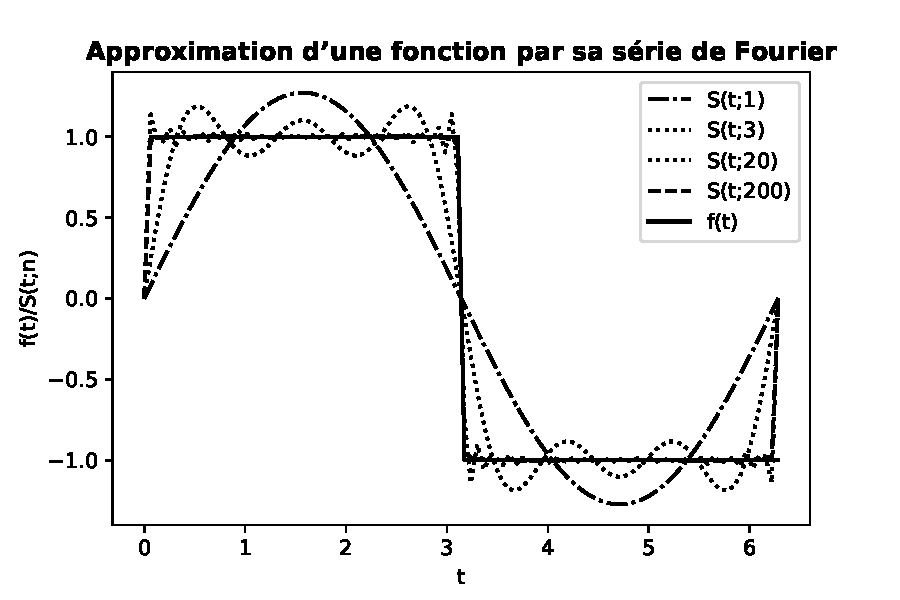
\includegraphics[width=1.0\linewidth]{imgs/fourier.pdf}}

\vspace{6mm}




% --- begin solution of exercise ---
\paragraph{Solution.}
Le programme qui donne le graphique est:
\begin{cod}{cbg_gray}\begin{minted}[fontsize=\fontsize{9pt}{9pt},linenos=false,mathescape,baselinestretch=1.0,fontfamily=tt,xleftmargin=2mm]{python}
plt.plot(t, S(t, n=1, T=2*pi), 'k-.', label = "S(t;1)")
plt.plot(t, S(t, n=3, T=2*pi), 'k:', label = "S(t;3)")
plt.plot(t, S(t, n=20, T=2*pi), 'k:', label = "S(t;20)")
plt.plot(t, S(t, n=200, T=2*pi), 'k--', label = "S(t;200)")
plt.plot(t, F, 'k-', label = "f(t)")
plt.title(u"Approximation d’une fonction par sa série de Fourier", fontweight='bold')
plt.ylabel("f(t)/S(t;n)")
plt.xlabel("t")
plt.legend()
\end{minted}
\end{cod}
\noindent

% --- end solution of exercise ---

\subex{f)}
Quelle est la relation entre la qualité de l'approximation et le choix de la valeur de \texttt{n}?


% --- begin solution of exercise ---
\paragraph{Solution.}
La qualité de l'approximation dépend de $n$. $S(t;n)\rightarrow f(t)$ quand $n\rightarrow\infty$.

% --- end solution of exercise ---

\end{doconceexercise}
% --- end exercise ---


% !split


% --- begin exercise ---
\begin{doconceexercise}
\refstepcounter{doconceexercisecounter}

\exercisesection{Exercise \thedoconceexercisecounter: Fonctions spéciales (intégrales de Fresnel et spirale de Cornu)}


Les intégrales de Fresnel ont été introduites par le physicien français Augustin Fresnel (1788-1827) lors de ses travaux sur les interférences lumineuses (voici un article intéressant à lire: \href{{http://www.mathouriste.eu/Fresnel/Fresnel.html}}{Fresnel, des Mathématiques en Lumière}).

Ces intégrales doivent être calculées numériquement à partir des développements en série des intégrales:

$$\int_{0}^{x} e^{-i\frac{\pi t^{2}}{2}} dt = \int_{0}^{x} cos(t^2) dt -i \int_{0}^{x} sin(t^2) dt= C(x) -i S(x)$$

Les fonctions de Fresnel sont des fonctions spéciales, définies par:

Pour $x \geq \sqrt{\frac{8}{\pi}}$
\begin{equation*}
\begin{aligned}
C(x) &= \frac{1}{2} + \cos\left(\frac{\pi x^{2}}{2}\right) gg1 + \sin\left(\frac{\pi x^{2}}{2}\right) ff1\\
S(x) &=  \frac{1}{2} - \cos\left(\frac{\pi x^{2}}{2}\right) ff1 + \sin\left(\frac{\pi x^{2}}{2}\right) gg1
\end{aligned}
\end{equation*}
et pour $0 \leq x < \sqrt{\frac{8}{\pi}}$
\begin{equation*}
\begin{aligned}
C(x) &= \cos\left(\frac{\pi x^{2}}{2}\right) gg2 + \sin\left(\frac{\pi x^{2}}{2}\right) ff2 \\
S(x) &= - \cos\left(\frac{\pi x^{2}}{2}\right) ff2 + \sin\left(\frac{\pi x^{2}}{2}\right) gg2
\end{aligned}
\end{equation*}
Où:
\begin{equation*}
\begin{aligned}
ff1 = \sum\limits_{n=0}^{11} \frac{d_{n}}{x^{2n+1}}\left(\frac{8}{\pi}\right)^{n+1/2} & gg1 = \sum\limits_{n=0}^{11} \frac{c_{n}}{x^{2n+1}}\left(\frac{8}{\pi}\right)^{n+1/2}\\
ff2 = \sum\limits_{n=0}^{11} b_{n}x^{2n+1}\left(\frac{\pi}{8}\right)^{n+1/2} & gg2 = \sum\limits_{n=0}^{11} a_{n}x^{2n+1}\left(\frac{\pi}{8}\right)^{n+1/2}
\end{aligned}
\end{equation*}
et $a_n$, $b_n$, $c_n$ et $d_n$ sont des coefficients tabulés  (\href{{https://www.ams.org/journals/mcom/1960-14-072/S0025-5718-1960-0121973-3/S0025-5718-1960-0121973-3.pdf}}{*J.Boersma Math Computation 14,380(1960)*}) et donnés dans un fichier \textbf{coef.dat}:

\begin{cod}{cbg_gray}\begin{minted}[fontsize=\fontsize{9pt}{9pt},linenos=false,mathescape,baselinestretch=1.0,fontfamily=tt,xleftmargin=2mm]{text}
#--------------------------------------------------
#    an            bn          cn           dn
#--------------------------------------------------
+1.595769140 -0.000000033 -0.000000000 +0.199471140
-0.000001702 +4.255387524 -0.024933975 +0.000000023
-6.808568854 -0.000092810 +0.000003936 -0.009351341
-0.000576361 -7.780020400 +0.005770956 +0.000023006
+6.920691902 -0.009520895 +0.000689892 +0.004851466
-0.016898657 +5.075161298 -0.009497136 +0.001903218
-3.050485660 -0.138341947 +0.011948809 -0.017122914
-0.075752419 -1.363729124 -0.006748873 +0.029064067
+0.850663781 -0.403349276 +0.000246420 -0.027928955
-0.025639041 +0.702222016 +0.002102967 +0.016497308
-0.150230960 -0.216195929 -0.001217930 -0.005598515
+0.034404779 +0.019547031 +0.000233939 +0.000838386
\end{minted}
\end{cod}
\noindent


Écrire un programme Python qui calcule les fonctions de Fresnel $C(x)$ et $S(x)$ ainsi que leurs représentations graphiques:


\subex{a)}
Définir les fonctions \texttt{ff1(x)}, \texttt{gg1(x)}, \texttt{ff2(x)} et \texttt{gg2(x)}. Chaque fonction renvoie la valeur de la somme qui lui correspond.


% --- begin solution of exercise ---
\paragraph{Solution.}
Les fonctions \texttt{ff1(x)}, \texttt{gg1(x)}, \texttt{ff2(x)} et \texttt{gg2(x)} sont les suivantes:
\begin{cod}{cbg_gray}\begin{minted}[fontsize=\fontsize{9pt}{9pt},linenos=false,mathescape,baselinestretch=1.0,fontfamily=tt,xleftmargin=2mm]{python}
# Importation
import numpy as np

def ff1(x):
    S = 0
    for i in range(12):
        fn = (8 / np.pi)**(i + 0.5) * dn[i]
        S += fn * x**(-2 * i - 1)
    return S

def gg1(x):
    S = 0
    for i in range(12):
        gn = (8 / np.pi)**(i + 0.5) * cn[i]
        S += gn * x**(-2 * i - 1)
    return S

def ff2(x):
    S = 0
    for i in range(12):
        fn = (np.pi / 8)**(i + 0.5) * bn[i]
        S += fn * x**(2 * i + 1)
    return S

def gg2(x):

    S = 0
    for i in range(12):
        gn = (np.pi/8)**(i + 0.5) * an[i]
        S +=  gn * x**(2 * i + 1)
    return S
\end{minted}
\end{cod}
\noindent

% --- end solution of exercise ---

\subex{b)}
Définir les fonctions Python \texttt{C(x)} et \texttt{S(x)} qui renvoient respectivement les listes, les valeurs de $C(x)$ et $S(x)$, \texttt{CF} et` SF` (en utilisant une boucle \texttt{for} pour remplir les listes par exemple).


% --- begin solution of exercise ---
\paragraph{Solution.}
Les fonctions Python \texttt{C(x)} et \texttt{S(x)} sont les suivantes:

\begin{cod}{cbg_gray}\begin{minted}[fontsize=\fontsize{9pt}{9pt},linenos=false,mathescape,baselinestretch=1.0,fontfamily=tt,xleftmargin=2mm]{python}
def C(x):
    CF=[]
    for i in range(len(x)):
        if x[i] >= np.sqrt(8/np.pi):
            cf=0.5 + np.cos((np.pi*x[i]**2)/2)*gg1(x[i]) + np.sin((np.pi*x[i]**2)/2)*ff1(x[i])
            CF.append(cf)
        elif 0 <= x[i] < np.sqrt(8/np.pi):
            cf = np.cos((np.pi*x[i]**2)/2)*gg2(x[i]) + np.sin((np.pi*x[i]**2)/2)*ff2(x[i])
            CF.append(cf)
    return CF
def S(x):
    SF=[]
    for i in range(len(x)):
        if x[i] >= np.sqrt(8/np.pi):
            sf = 0.5 - np.cos((np.pi*x[i]**2)/2)*ff1(x[i]) + np.sin((np.pi*x[i]**2)/2)*gg1(x[i])
            SF.append(sf)
        elif 0 <= x[i] < sqrt(8/np.pi):
            sf = -np.cos((np.pi*x[i]**2)/2)*ff2(x[i]) + np.sin((np.pi*x[i]**2)/2)*gg2(x[i])
            SF.append(sf)
    return SF
\end{minted}
\end{cod}
\noindent

% --- end solution of exercise ---

\subex{c)}
Créer des tableaux \texttt{an}, \texttt{bn}, \texttt{cn} et \texttt{dn} à partir du fichier \textbf{coef.dat}.


% --- begin solution of exercise ---
\paragraph{Solution.}
Les tableaux \texttt{an}, \texttt{bn}, \texttt{cn} et \texttt{dn} sont chargés  à partir du fichier \textbf{coef.dat} à l'aide del a fonction \texttt{numpy.loadtxt()}:
\begin{cod}{cbg_gray}\begin{minted}[fontsize=\fontsize{9pt}{9pt},linenos=false,mathescape,baselinestretch=1.0,fontfamily=tt,xleftmargin=2mm]{python}
an, bn, cn, dn = np.loadtxt('coef.dat', comments='#', usecols=(0, 1, 2, 3), unpack=True)
\end{minted}
\end{cod}
\noindent

% --- end solution of exercise ---

\subex{d)}
Créer un tableau \texttt{x}. Utilisez 800 intervalles pour évaluer les points dans [0,10] (cas où $x \geq 0$).


% --- begin solution of exercise ---
\paragraph{Solution.}
Le tableau \texttt{x} s'écrit:
\begin{cod}{cbg_gray}\begin{minted}[fontsize=\fontsize{9pt}{9pt},linenos=false,mathescape,baselinestretch=1.0,fontfamily=tt,xleftmargin=2mm]{python}
x = np.linspace(0,10, 500)
\end{minted}
\end{cod}
\noindent

% --- end solution of exercise ---

\subex{e)}
Transformer \texttt{C(x)} et \texttt{S(x)} en tableaux \texttt{numpy}, respectivement \texttt{CF} et \texttt{SF}.


% --- begin solution of exercise ---
\paragraph{Solution.}
Les listes \texttt{C(x)} et \texttt{S(x)} sont transformés en tableaux \texttt{numpy} à l'aide de la fonction \texttt{numpy.array()}:
\begin{cod}{cbg_gray}\begin{minted}[fontsize=\fontsize{9pt}{9pt},linenos=false,mathescape,baselinestretch=1.0,fontfamily=tt,xleftmargin=2mm]{python}
CF = np.array(C(x)); SF = np.array(S(x))
\end{minted}
\end{cod}
\noindent

% --- end solution of exercise ---

\subex{f)}
Tracer une grille de figures à 2 colonnes (voir Cours3: \href{{https://codetunisia.github.io/CoursSimNum/cours3/md/cours3.html#linstruction-subplot}}{Vues en grille}) dont le graphique de gauche représente \texttt{CF} et \texttt{SF} en fonction de \texttt{x} et le graphique de droite représente une \href{{https://fr.wikipedia.org/wiki/Clotho%C3%AFde}}{clothoïde} (ou spirale de Cornu, ou Spirale de Fresnel..)`SF` en fonction de \texttt{CF}.
La sortie de ce programme devrait être comme suit:


\vspace{6mm}

% inline figure
\centerline{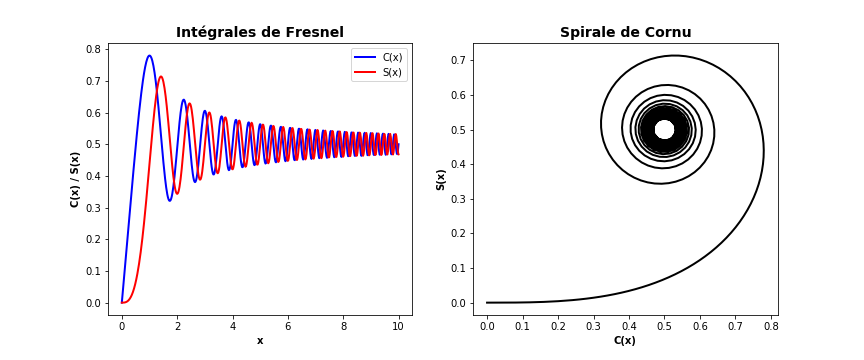
\includegraphics[width=1.0\linewidth]{imgs/fresnel.png}}

\vspace{6mm}




% --- begin solution of exercise ---
\paragraph{Solution.}
La représentation graphique des intégrales de Fresnel et du spirale de Cornu est donc:
\begin{cod}{cbg_gray}\begin{minted}[fontsize=\fontsize{9pt}{9pt},linenos=false,mathescape,baselinestretch=1.0,fontfamily=tt,xleftmargin=2mm]{python}
plt.figure(figsize=(12,5))
subplot(1,2,1)
plt.plot(x, CF,'b', x, SF,'r', linewidth=2)
plt.xlabel("x", fontweight='bold'); plt.ylabel("C(x) / S(x)", fontweight='bold')
plt.title(u"Intégrales de Fresnel", fontsize=14, fontweight='bold')
plt.legend(["C(x)","S(x)"])
subplot(1,2,2)
plt.plot(CF, SF, linewidth = 2, color = 'k')
plt.xlabel("C(x)", fontweight='bold'); plt.ylabel("S(x)", fontweight='bold')
plt.title("Spirale de Cornu", fontsize=14, fontweight='bold')

plt.savefig("fresnel.png")
plt.show()
\end{minted}
\end{cod}
\noindent

% --- end solution of exercise ---

\end{doconceexercise}
% --- end exercise ---


% ------------------- end of main content ---------------

% #ifdef PREAMBLE
\end{document}
% #endif

